% Charlotte Geiger - Manuel Lippert - Leonard Schatt
% Physikalisches Praktikum

% 2.Kapitel Fragen zur Vorbereitung

\chapter{Fragen zur Vorbereitung}
\label{chap:fvz}
\section{Eingangs- und Ausgangsimpedanz eines Hochpass}
Die Definition einer Eingangsimpedanz ist der Widerstand am Eingang eines Gerätes. Niedrige Ausgangsimpedanzen ermöglichen lange Kabelwege ohne Beeinträchtigung\\
Bei Frage 1 wird nach der Eingangs- und Ausgangsipedanz des komplexen Spannungsteiler in folgender Abb. 2.1 gefragt.
\begin{center}
    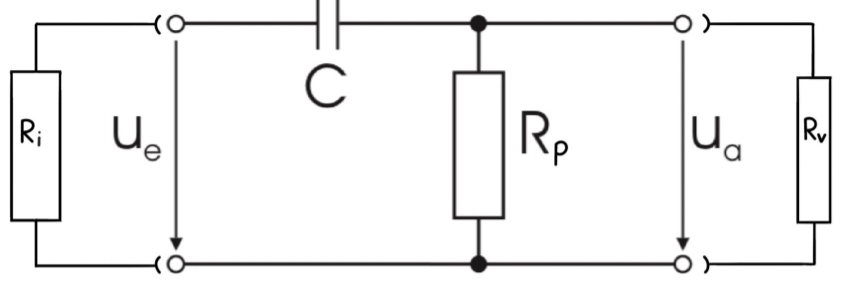
\includegraphics[scale=0.5]{Hochpass.PNG}
    \captionof{figure}{Hochpass als komplexer Spannungsteiler}
\end{center}
Zuerst wird der komplexe Widerstand von der Eingangsimpedanz berechnet. So gilt nach den Kirkoff'schen Regeln des Widerstandsnetzes:
\begin{equation}
    \begin{aligned}
        Z_e &= \frac{1}{\frac{1}{R_i}+\frac{1}{R_C+{\frac{1}{R_V}+\frac{1}{R_P}}}}\\[0.3cm]
        \xrightarrow{R_C=\frac{1}{i\omega C}}~Z_e &=\frac{R_i(R_V+R_P+i\omega C(R_VR_P))}{R_V+R_P+i\omega C(R_VR_i+R_PR_i+R_VR_P)}\\[0.3cm]
        &= \frac{R_V+R_P+i\omega C(R_VR_P)}{\frac{1}{R_i}(R_V+R_P+i\omega C(R_VR_P))+i\omega C(R_V+R_P)}\\
    \end{aligned}
\end{equation}
Da der Innenwiderstand der Eingangs-Spannungsquelle vernachlässigt werden kann, nimmt man an, dass $R_i$ gegen unendlich geht.\\
\begin{align}
    \xrightarrow{R_i\rightarrow\infty}~Z_e=\frac{R_V+R_P+i\omega C(R_VR_P)}{i\omega C(R_V+R_P)}
\end{align}
Für Impendanz ohne Last $(R_V\longrightarrow\infty)$:
\begin{align}
    Z_e=\frac{1+\frac{R_P}{R_V}+i\omega C R_P}{i\omega C(1+\frac{R_P}{R_V})}~\xrightarrow{R_V\rightarrow\infty}~Z_e=\frac{1+i\omega CR_P}{i\omega C} = R_P+\frac{1}{i\omega C}
\end{align}
Diese Lösungsformel beschreibt die Reihendarstellung von Kondensator und Widerstand. \\
Nun wird die der komplexe Widerstand der Ausgangsimpedanz betrachtet. Man geht analog zu oben vor, jedoch beginnt man bei der Betrachtung der Widerstandsreihenfolge auf der rechten Seite des Schaltbildes. 
\begin{align}
    Z_a=\frac{1}{\frac{1}{R_V}+\frac{1}{R_P}+\frac{1}{R_i+\frac{1}{i\omega C}}}=\frac{R_VR_P(i\omega CR_i+1)}{R_P+R_V+i\omega C(R_VR_P+R_PR_i+R_iR_V)}
\end{align}
Analog zu oben:
\begin{align}
    \begin{aligned}
        \text{Innenwiderstand vernachlässigbar:}&~\xrightarrow{R_i\longrightarrow\infty}~Z_a=\frac{R_VR_P}{R_P+R_V}=\frac{1}{\frac{1}{R_V}+\frac{1}{R_P}}\\
        \text{Impedanz ohne Last:}&~\xrightarrow{R_V\rightarrow\infty}~Z_a=R_P
    \end{aligned}
\end{align}
Bei solch einer Schaltung werden hochfrequente Eingangsspannungen $U_e$ am Ausgang ungehindert durchgelassen, weshalb die Schaltung Hochpass genannt wird.
\section{Beschriftung Oszilloskop und Kabelimpedanz}
Kabelimpedanz (auch Leistungswellenwiderstand) ist einer von vielen Parametern bzw.
Kenngrößen von längshomogenen Leitungen und steht synonym zum komplexen Widerstand.
Der Strom, der nötig ist, um das Ende des Kabels bzw. Leitung auf der Spannung U zu halten hängt linear von U ab und gleicht daher echten Widerstand. Das ist also auch die charakteristische Impedanz einer Leitung, wenn man von eimen "50-$\Omega$-Kabel" spricht.\\
Wenn am Eingang eines Oszilloskops "1M$\Omega$, 20pF" vermerkt ist, bedeutet dies die Eingangsimpedanz. Die Eingangsimpedanz eines Oszilloskops sagt aus, wie groß der komplexe Widerstand des Kanaleingangs ist, wird in Ohm und Fahrrad getrennt angegeben und erfolgt meist als Aufdruck neben der Kanaleingangsbuchse am Oszilloskop. Übliche Werte für die Impedanz sind 1M$\Omega$ und 10 bis 25pF für die Parallelkapazität. Die Angabe liegt also in der Norm von Oszillatoren.
\section{Transistor - Funktionsweise und Aufbau}
Der Transistor ist ein Halbleiterbauelement, das in einer elektrischen Schaltung verbaut ist.
Über den Transistor kann man die Ströme in dem Stromfluss so beeinflussen, dass überhaupt
kein Strom fließt (er fungiert als Schalter), oder man kann den Fluss verstärken bzw.
beschleunigen, wodurch deutlich stärkerer Strom fließt (er fungiert als Verstärker).\\
Jeder Transistor besteht aus drei dünnen übereinandergelegten Halbleiterschichten, die mit
metallischen Anschlüssen versehen sind. Die drei Anschlüsse sind: die Basis (B), der Kollektor
(C) und der Emitter (E).\\
Es wird je nach Reihenfolge der Dotierung zwischen NPN- Transistor und PNP-Transistor
unterschieden. Zweiterer besteht aus zwei p-leitenden Schichten zwischen denen eine dünne
n-leitende Schicht liegt. Im Schaltkreis ist dies so gekennzeichnet, dass der Pfeil des Emitters
zur Basis hin zeigt. 
Dotierung bedeutet das Einbringen von Fremdatomen bei dem Herstellungsprozess in eine Schicht des hochreinen Halbleitermaterials, um die Kristallstruktur zu verändern. Somit kann durch äußeren Einfluss Ladungsträger verschoben werden.\\
Die konkrete Funktion von Transistoren beruht auf freien Ladungsträgern beim Emitter. Durch
eine angelegte Spannung zwischen Basis und Emitter wird eine Sperrschicht abgebaut und die
Ladungsträger wandern in die Basis-Zone. Ein kleiner Steuerstrom auf der
Basis-Emitter-Strecke führt zu Raumladungszonenveränderungen im Inneren des
Bipolartransistors, wodurch ein großer Strom auf der Kollektor-Emitter-Strecke gesteuert
werden kann. Konkret beim PNP-Transistor: Der Emitter (p-dotiert) hat Löcher als freie Ladungsträger. Bei positiver Spannung zwischen Basis und Emitter wird die Sperrschicht dazwischen abgebaut und die "Löcher wandern" in die Basis Zone. Die eingedrungenen Ladungsträger werden nun vom starken elektrischen Feld in Richtung Kollektor beschleunigt.
Bipolartransistoren sind grundsätzlich immer selbstsperrend: Ohne Ansteuerung mittels eines
kleinen Stromes durch die Basis-Emitter-Strecke sperrt der Transistor auf der
Kollektor-Emitter-Strecke\\
\begin{center}
    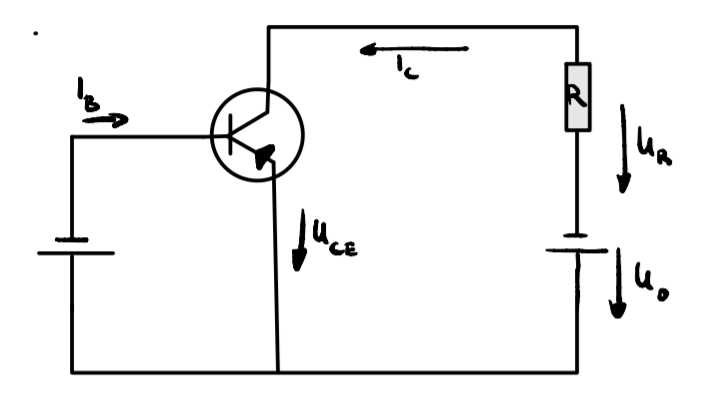
\includegraphics[scale=0.5]{PNP-Transistor.PNG}
    \captionof{figure}{pnp-Transistor in Emitterschaltung}
\end{center}
Im folgenden werden die Eigenschaften eines bipolaren PNP-Transistors
aufgelistet/zusammengefasst:
\begin{enumerate} 
\item Der Transistor wirkt wie ein elektrisch gesteuerter Widerstand. DIe Ursache dabei ist die
Basisstromänderung, wodurch auch der Kollektorstrom sich verändert. Dieser fließt nur,
wenn auch ein Basisstrom fließt.
\item Der Kollektorstrom ist um ein Vielfaches größer als der Basisstrom, der Unterschied
rührt von der Aufteilung des Elektronenflusses von Kollektor und Basis.
\item Der Basisstrom fließt erst, wenn die Schwellspannung an der Basis-Emitter-Strecke
überwunden ist. Wenn der Basisstrom nicht fließt, dass sperrt der Transistor
\item Der bipolare Transistor hat zwei Stromkreise, der dieser vereint. Den Steuerstromkreis
und den Arbeits-bzw. Laststromkreis.
\end{enumerate}
\section{Ein- und Ausgangskennlinien}
Der Zusammenhang zwischen relevanten Werten des Transistors wird in Kennlinienfeldern dargestellt. 
Kennlinienfelder sind Diagramme, in denen der Kollektorstrom als Funktion der Kollektorspannung aufgetragen wird, da der Zusammenhang abhängig von der Basis-Stromstärke ist, gibt es mehrere Kennlinien in dem Kennlinienfeld. Bei bipolaren Transistoren, die als Schalter oder Verst\"arker genutzt werden, reichen 4 Kennlinienfelder aus, der Zusammenhang aller relevanter Werte wird dann in einem sogenannten Vierquadrantenkennlinienfeld dargestellt. \\
\begin{enumerate} 
\item Eingangskennlinien(-feld)\\
Als Eingangskennlinie wird die Funktion $I_B(U_{BE})$ benannt und ist von der Temperatur abhängig. Je höher die Temperatur, desto  größer die Eigenleitfähigkeit des Halbleiterkristalls. Dann leitet die Basis-Emitterstrecke schon bei kleineren Steuerspannungen und bewirkt einen höheren Basisstrom. \\
Bei Auswertung des Basisstroms als Funktion der Basis-Emitterspannung im Diagramm, so zeigt sich die Durchlasslinien einer SI-Diode. 
\item Ausgangskennlinien(-feld)
Ausgangskennlinien werden als Funktion von $I_C(U_{CE})$ beschrieben. Im Ausgangskennlinienfeld wird die Abhängigkeit des Kollektorstroms von der Kollektor-Emitterspannung bei konstantem Basissteuerstrom dargestellt. 
\end{enumerate}
Wie oben schon beschrieben kann man verschiedene Kennlinienfelder zu einem kompakten Feld zusammenschließen, wodurch es deutlich übersichtlich wird. Weitere Kennlinienfelder sind Spannungsrückwirkungs- und Stromverstärkungskennlinienfelder
\section{Emitter-, Basis- und Kollektorschaltung}
\begin{center}
    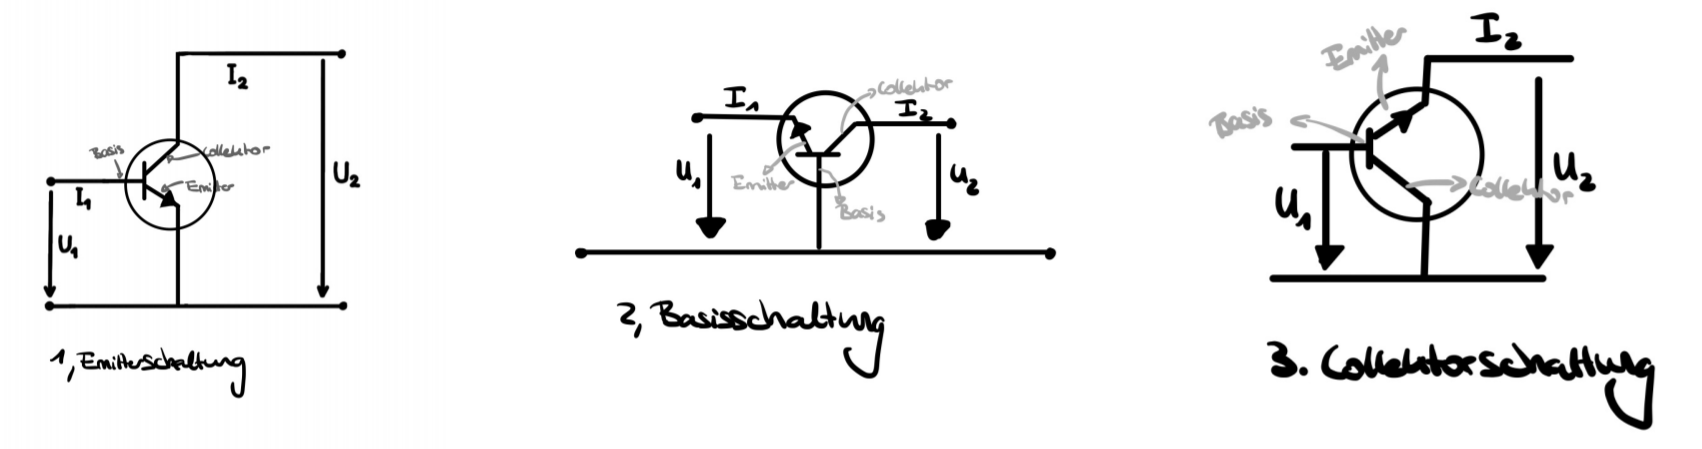
\includegraphics[scale=0.4]{Schaltungstypen.PNG}
    \captionof{figure}{Schaltungstypen}
\end{center}
Im folgenden werden kurz die herausstechenden Unterschiede der drei Schaltungstypen
umrissen. Ausschlaggebend sind Ein- und Ausgangswiderstand, sowie Strom-, Spannungs- und
Leistungsverstärkung.
\begin{enumerate} 
\item Emitterschaltung\\
Diese Schaltung ist mit Abstand die am häufigsten verwendete Schaltung im
Niederfrequenzbereich. Sie ist eine Universal-Verstärkungsschaltung, die zur Erzeugung sehr hoher Spannungsverstärkungen genutzt wird. Jedoch ist die Schaltung sehr frequenzabhängig, je höher die Frequenz, desto niedriger die Verstärkung. \\
Bei dieser Schaltung wird das zu verstärkende Signal an die Basis angelegt
und das Ausgangssignal am Kollektor abgegriffen. Der Verstärkungsfaktor und der
Ausgangswiderstand sind in dieser Schaltung hoch. Die Emitterschaltung besteht vor allem aus dem Kollektorwiderstand $R_C$, einem Transistor, der Eingangssignalquelle $U_e$ mit dem Basis-Vorwiderstand $R_V$ oder einem Spannungsteiler $(R_1 und R_2)$ unf der Betriebsspannung $U_B$. Ausgangspunkt für die Ausgangsspannung $U_a$ ist der Kollektoranschluss des Transistors. Gemeinsame Bezugspunkt von Eingangs- und Ausgangsspannung ist der Emitteranschluss. Daher auch der Name der Emitterschaltung. 
\item Basisschaltung\\
Durch $U_1<<U_2$ und $I_1>=I_2$ folgt eine schwache Stromverstärkung, aber eine hohe
Spannungsverstärkung. Bei der Basisschaltung ist die Besonderheit, dass der Basisanschluss des Transistors durch einen Kondensator wechselstrommäßig an Masse liegt. Die Stromverstärkung einer Basisschaltung ist immer kleiner als 1. Sie erreicht diesen Wert genau dann, wenn der Arbeitswiderstand groß gegen den Lastwiderstand ist.  
Die Anwendungsbereiche dieser Schaltung ist vorzugsweise bei Hochfrequenz-Verstärkern. Die kapazitative Belastung einer hochfrequenten Signalquelle ist sehr gering, wodurch der Verstärker eine große Bandbreite besitzt. 
\item Kollektorschaltung\\
Diese Schaltung entspricht dem Schaltaufbau einer Emitterschaltung nur ohne Kollektorwiderstand. 
$I_1<<I_2$ und $U_1>=U_2$ Daraus folgt dass der Eingangswiderstand hoch ist und der
Ausgangswiderstand niedrig. Damit folgt eine hohe Stromverstärkung und eine niedrige
Spannungsverstärkung.
Dieses Schaltbild eignet sich hervorragend als Impedanzwandler bzw. Spannungsverstärker, wegen der hohen Eingangs- und niedrigen Ausgangsimpedanzen der Schaltung. 
\end{enumerate}
\section{Emitterschaltung}
\begin{center}
    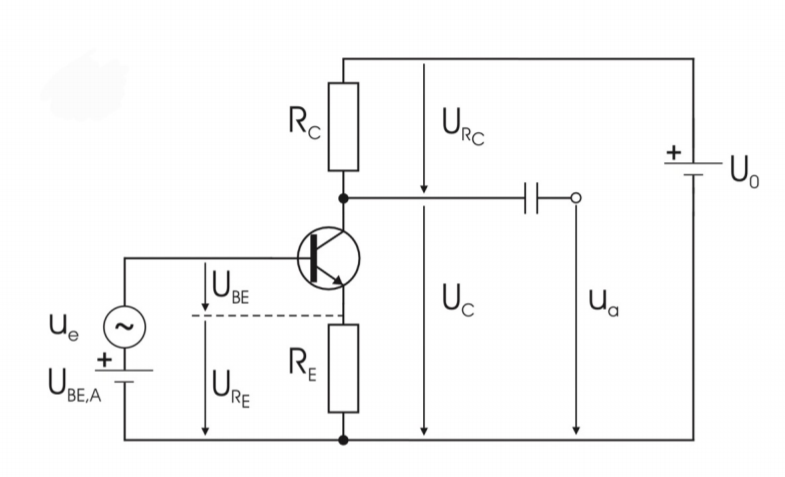
\includegraphics[scale=0.5]{Emmitterschaltung.PNG}
    \captionof{figure}{Emitterschaltung mit Stromgegenpolung}
\end{center}
Es soll die Gleichung (6) aus dem Skript hergelitten werden.
\begin{align}
    v=\frac{u_a}{u_e}= -\frac{R_C}{(\frac{r_{BE}}{ \beta }+R_E)} \approx -\frac{R_C}{R_E}
\end{align}
Wobei $v=\frac{u_a}{u_e}$ der Spannungsverst\"arker ist.\\
Bereits bekannt ist 
$u_a= -i_CR_C$ und $u_e=i_Br_{BE}$. Mit Einf\"ugen des Widerstandes $R_E$ wird $u_e$ zu $u_e=i_Br_{BE}+i_ER_E$
Somit ergibt sich folgendes:
\begin{align}
    v=\frac{-i_CR_C}{i_Br_{BE}+i_CR_E}
\end{align}
Mit dem Umstellen der differentiellen Stromverst\"arkung  $\beta = \frac{i_C}{i_B}$ bekommt man den Ausdruck:
\begin{align}
    v=-\frac{i_CR_C}{i_Cr_{BE}+i_ER_E}
\end{align}
Mit dem Zusammenhang $i_C\sim i_E$ und nach k\"urzen von $i_C$ bekommt man die Gleichung (6):
\begin{align}
    v=-\frac{R_C}{\frac{r_{BE}}{\beta}+R_E}
\end{align}
Mit der Annahme, dass $R_E$ deutlich gr\"o\ss{}er als $r_{BE}$ ist, erkennt man, dass
\begin{align}
    v=\frac{u_a}{u_e} \approx -\frac{R_C}{R_E} \tab \Rightarrow \tab r_e=r_{BE}= \beta R_E~\text{und}~r_a\approx R_C
\end{align}

\section{Allgemeines}
Die Erfindung des Transistors revolutionierte die Menschheit so wie kaum eine andere
Erfindung.
Erfunden wurde der Transistor von Julius Edgar Lilienfeld 1925, der in seiner Arbeit ein
elektronisches Bauelement beschreibt, das Elektronenröhreneigenschaften aufweist.
Es gibt zwei Verschiedene Arten von Transistoren. Zum einen den Feldeffekttransistor (FET)
(unipolare Transistoren) oder den Bipolartransistor (BJT)
Die Bezeichnung Transistor wird abgeleitet von transfer resistor, da bei Widerstandsänderung in Schicht A
einer Halbleiterschicht auch der Widerstand in einer Schicht B beeinflusst wird.
Bipolare Transistoren bestehen heutzutage üblicherweise aus Silizium. Der Grund weshalb heutzutage mehr Silizium-Transistoren als Germanium-Transistoren verwendet werden, ist zum Einen die unterschiedliche Beschaffenheit der Materialien. So bricht Germanium bei einer Temperatur von 82 Grad und ist daher nicht sehr Hitzebest\"andig und bei Silizium ist dies nicht der Fall und zus\"atzlich sch\"utzen Oxide das Silizium und isolieren das Bauteil. Auch ist Silizium als Elementarhalbleiter deutlich einfacher zu gewinnen und zu handhaben. 